% System overview drawn from one real record: FF++ test frame 454 with the mouth replaced from a donor (part-level forgery,
% held out). Tiles and numbers come from make_tiles_arch.py (arch_*.png, arch_numbers.tex). Fonts are the document's.
% Geometry: tiles 1.9 cm tall (1.68 cm wide), one short label per tile (details in the caption), row B 5.2 cm below row A.
\newcommand{\pReal}{0.00}
\newcommand{\pFake}{1.00}
\newcommand{\pBeau}{0.00}
\newcommand{\evEyes}{0.02}
\newcommand{\evNose}{0.41}
\newcommand{\evMouth}{0.99}
\newcommand{\evSkin}{0.28}
\newcommand{\evContour}{0.03}
\newcommand{\namedPart}{mouth}
\newcommand{\opEye}{0.24}
\newcommand{\opSlim}{0.10}
\newcommand{\opWhite}{0.13}
\newcommand{\opSmooth}{0.10}

\begin{tikzpicture}[
  font=\footnotesize, >={Latex[length=2.2mm,width=1.8mm]},
  tile/.style={inner sep=0pt, outer sep=0pt},
  lab/.style={font=\footnotesize, text=ink, align=center, text width=1.95cm, inner sep=0pt},
  arr/.style={->, line width=0.9pt, draw=ink},
  card/.style={draw=#1, fill=#1!5, rounded corners=3pt, line width=0.7pt, inner sep=5pt, align=left, text=ink},
]
\definecolor{nn}{HTML}{0F4D92}
\definecolor{code}{HTML}{1B7F4C}
\definecolor{chk}{HTML}{6A3D9A}
\definecolor{ink}{HTML}{222222}
\definecolor{muted}{HTML}{6B6B6B}
\definecolor{track}{HTML}{E5E5E5}
\definecolor{fk}{HTML}{D55E00}
\definecolor{rl}{HTML}{009E73}
\definecolor{bt}{HTML}{C98A00}
\def\TH{1.9cm}

% ================= row A: photo -> crop -> backbone -> heads -> map =================
\node[tile, anchor=west] (photo) at (0,0) {
\includegraphics[height=\TH]{figs/arch_photo.png}};
\node[lab, below=3pt of photo] {\textcolor{code}{\textbf{1}} photo,\\landmarks};
\node[tile, right=0.45cm of photo] (crop) {
\includegraphics[height=\TH]{figs/arch_crop.png}};
\node[lab, below=3pt of crop] {\textcolor{code}{\textbf{2}} aligned\\crop};

\node[inner sep=0pt, outer sep=0pt, minimum width=1.3cm, minimum height=\TH, right=0.45cm of crop] (bb) {};
\draw[draw=nn, fill=nn!15, line width=0.8pt]
  ($(bb.west)+(0,-0.95cm)$) -- ($(bb.west)+(0,0.95cm)$) -- ($(bb.east)+(0,0.55cm)$) -- ($(bb.east)+(0,-0.55cm)$) -- cycle;
\node[font=\footnotesize, text=nn, align=center] at (bb) {back-\\bone};
\node[lab, below=3pt of bb, text width=1.9cm] {\textcolor{nn}{\textbf{3}} CLIP or\\EfficientNet};

\node[card=nn, right=0.45cm of bb, minimum height=\TH, minimum width=4.2cm, inner sep=0pt, anchor=west] (heads) {};
\node[lab, below=3pt of heads, text width=4.4cm] {\textcolor{nn}{\textbf{4}} heads: class scores,\\operation scores, map};
\coordinate (h0) at ($(heads.west)+(1.6cm,0.5cm)$);
\foreach \y/\name/\val/\col in {0/real/\pReal/rl, 1/fake/\pFake/fk, 2/beautified/\pBeau/bt} {
  \node[anchor=east, font=\footnotesize, text=ink, inner sep=0pt] at ($(h0)+(-0.1cm,-\y*0.5cm)$) {\name};
  \fill[track] ($(h0)+(0,-\y*0.5cm-0.12cm)$) rectangle ($(h0)+(1.5cm,-\y*0.5cm+0.12cm)$);
  \fill[\col] ($(h0)+(0,-\y*0.5cm-0.12cm)$) rectangle ($(h0)+(1.5cm*\val+0.02cm,-\y*0.5cm+0.12cm)$);
  \node[anchor=west, font=\footnotesize, text=ink, inner sep=0pt] at ($(h0)+(1.6cm,-\y*0.5cm)$) {\val};
}

\node[tile, right=0.45cm of heads] (map) {
\includegraphics[height=1.3cm]{figs/arch_map16.png}};
\node[lab, below=3pt of map, text width=1.7cm] {evidence map\\$16{\times}16$};

\draw[arr] (photo) -- (crop);
\draw[arr] (crop) -- (bb);
\draw[arr] (bb) -- (heads);
\draw[arr] (heads) -- (map);

% training, once, offline (above the network)
\node[draw=nn, dashed, fill=white, rounded corners=3pt, line width=0.6pt, inner sep=4pt, text width=8.0cm, align=left, font=\footnotesize, text=ink,
      anchor=south west] at ($(bb.north west)+(-0.2cm,0.45cm)$) (trn)
  {\textcolor{nn}{\textbf{trained once, offline:}} genuine FF++ frames and FFHQ originals; forgeries and 61,510 part-level edits
   with exact footprints; renders of two retouching services. Skin smoothing is shown to \emph{both} classes.};
\draw[arr, dashed, draw=nn] (trn.south -| bb) -- (bb.north);

% ================= row B: map on the face -> parts -> named part -> sentences and checks =================
\node[tile, anchor=west] (ev) at (0,-5.2) {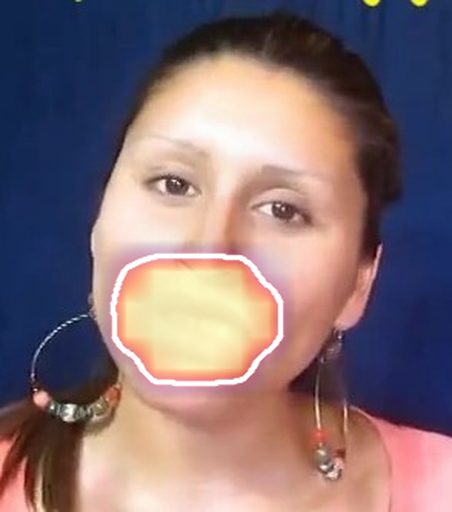
\includegraphics[height=\TH]{figs/arch_evidence.png}};
\node[lab, below=3pt of ev] {\textcolor{code}{\textbf{5}} map on\\the face};
\node[tile, right=0.45cm of ev] (parts) {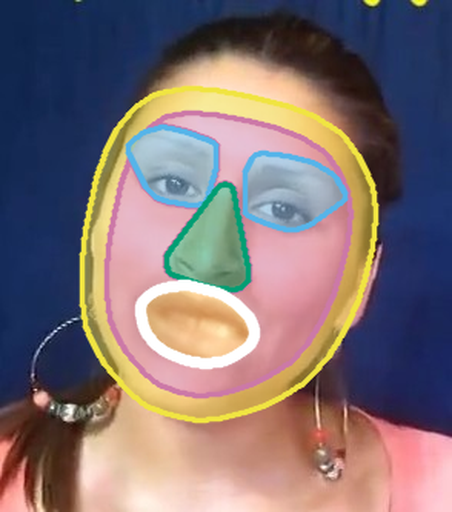
\includegraphics[height=\TH]{figs/arch_parts.png}};
\node[lab, below=3pt of parts] {\textcolor{code}{\textbf{6}} five part\\masks};
\node[tile, right=0.45cm of parts] (named) {
\includegraphics[height=\TH]{figs/arch_named.png}};
\node[lab, below=3pt of named, text width=2.1cm] {\textcolor{code}{\textbf{7}} named part:\\\namedPart\ \evMouth};

\node[card=code, text width=6.3cm, anchor=north west] (sen) at ($(named.north east)+(0.45cm,0)$)
  {The model's decision is \textbf{fake} (score \textbf{\pFake}). The evidence is concentrated on the \textbf{\namedPart}
   (mean evidence \textbf{\evMouth}). The score is the model's raw output, not a calibrated probability.\\[3pt]
   \textcolor{chk}{\textbf{checks}}\ \textcolor{rl}{\ding{51}} H1--H6 match the record\quad \textcolor{rl}{\ding{51}} G7--G9 no misuse of the score};
\node[lab, below=3pt of sen, text width=6.4cm] {\textcolor{code}{\textbf{8}} sentences from templates, numbers copied from the record;
  \textcolor{chk}{\textbf{9}} checked, then shown on the page (Figure~\ref{fig:output})};

\draw[arr] (ev) -- (parts);
\draw[arr] (parts) -- (named);
\draw[arr] (named.east) -- (named.east -| sen.west);
% from the map (end of row A) down and across to the face (start of row B)
\draw[arr] (map.south) -- ($(map.south |- ev.north)+(0,0.6cm)$) -| (ev.north);
\node[font=\footnotesize, text=muted, fill=white, inner sep=1.5pt] at ($(heads.south |- ev.north)+(0,0.6cm)$) {upsampled onto the crop};

% legend, under the lowest element (the card's label)
\node[anchor=north west, font=\footnotesize, text=muted, text width=13.8cm, align=left, inner sep=0pt] at ($(ev.west |- sen.south)+(0,-1.7cm)$)
  {\textcolor{nn}{\textbf{blue}} neural network\quad \textcolor{code}{\textbf{green}} code with fixed rules\quad
   \textcolor{chk}{\textbf{purple}} checks\quad steps 1--9 run in the browser; the photo never leaves the device};
\end{tikzpicture}
